\documentclass[11pt,a4paper]{article}
\usepackage{fontspec}
\setmainfont{TeX Gyre Pagella}
\newfontfamily\headfont{Inter}[UprightFont=*-ExtraBold,BoldFont=*-ExtraBold,Extension=.otf,Path=/usr/share/fonts/opentype/inter/]
\usepackage[a4paper,margin=2.3cm]{geometry}
\usepackage{graphicx,booktabs,float,caption,array,xcolor,longtable}
\usepackage{xurl}
\usepackage[hidelinks]{hyperref}
\usepackage{titlesec}
\usepackage[round]{natbib}
\usepackage{setspace}
\setstretch{1.05}
\renewcommand{\topfraction}{0.9}
\renewcommand{\bottomfraction}{0.8}
\renewcommand{\textfraction}{0.1}
\renewcommand{\floatpagefraction}{0.75}
\setlength{\parindent}{0pt}
\setlength{\parskip}{0.55em}
\titleformat{\section}{\headfont\Large}{\thesection}{0.8em}{}
\titleformat{\subsection}{\headfont\large}{\thesubsection}{0.8em}{}
\captionsetup{font=small,labelfont=bf}
\urlstyle{same}
\hypersetup{pdftitle={Where the Sun Sets into the Sea},pdfauthor={Tristan Hotham}}


\begin{document}
\begin{center}
{\Large\bfseries Where the Sun Sets into the Sea\par}
\vspace{0.4em}
{\large Sea sunsets and sunrises through the year at 1,717 beaches in Britain and Ireland\par}
\vspace{1.2em}
{\large Tristan Hotham\par}
\vspace{0.3em}
{\small Independent researcher\\
ORCID: 0000-0003-4931-9349\\
DOI: https://doi.org/10.5281/zenodo.24089892\par}
\vspace{0.8em}
2026
\end{center}

\begin{quote}
\small
\begin{center}\textbf{Abstract}\end{center}
From which beaches can one watch the Sun set into, or rise out of, the open sea, and on which days of the year? For the 1,717 named coastal beaches of the United Kingdom and Ireland in OpenStreetMap, I place an observer at the water's edge, eye 3 m above the sea, and cast rays every 0.25\textdegree{} across the year's sunrise and sunset bearings, out to 150 km. Within 12 km the sea is OpenStreetMap's coastline rasterised from OpenFreeMap vector tiles at about 20 to 25 m; beyond, land is terrain above sea level. Land blocks the Sun only where it rises above the sea horizon, allowing for the Earth's curvature and refraction. 46.9\% of beaches have a sea sunset on at least one day of 2026, 40.9\% a sea sunrise, 8.9\% both, and 21.0\% neither; 52 beaches, 43 of them in Cornwall, have a sea sunset every day. Sea views are commoner in winter than in summer (349 against 303 beaches for sunsets, 405 against 231 for sunrises on the solstices). Wales has the highest share of sea-sunset beaches (67\%). Islands hide the Sun on some days from 303 beaches at sunset and 179 at sunrise: the Isle of Wight and Mull from the most beaches (31 each), Arran from Troon on 134 days, Lundy from Woolacombe on 26.

\textbf{Keywords:} sunset; sunrise; horizon; beaches; coastline; viewshed; refraction; OpenStreetMap; Great Britain; Ireland
\end{quote}

\section{Introduction}
Whether the Sun sets over the sea is one of the first questions asked of a beach, and one of the least often answered with data. The answer depends on the bearing of sunset, which swings through about 90 to 110\textdegree{} of azimuth over the year at the latitudes of Britain and Ireland, on the shape of the coast (headlands, the far shore of a bay or firth), on islands, and on whether distant land stands above the curved sea horizon. This paper computes it for every named beach, day by day.

\section{Data}
\textbf{Beaches.} OpenStreetMap \citep{osm} features tagged \texttt{natural=beach} with a name in the United Kingdom and Ireland, with full geometry, queried with QLever \citep{qlever}: 1,826 features, merged into 1,768 beaches where features of the same name in the same country lie within 1 km. 51 beaches have no sea within 600 m (lake and river beaches) and are excluded, leaving 1,717 (1,282 in the United Kingdom, 435 in Ireland).

\textbf{Sea.} The \texttt{water} layer (class \texttt{ocean}) of the OpenFreeMap \citep{openfreemap} vector tiles, release 20261101\_080013\_pt, at zoom 10, which carries OpenStreetMap's coastline (mean high water); each tile was rasterised to 1,024 by 1,024 pixels, about 25 m at 50\textdegree N and 19 m at 60\textdegree N. Tiles were fetched one at a time, rasterised and deleted.

\textbf{Terrain.} The AWS Terrain Tiles at zoom 10 (about 90 m, with bathymetry below sea level) give land heights along the rays and the land beyond 12 km.

\section{Method}
\textbf{Observer.} Candidate points are sea pixels at least two pixels (about 40 to 50 m) from land, within three pixels of the nearest such pixel to the beach; up to twelve are spread along the beach and the one with the most open bearings within 3 km over the year's sunrise and sunset arcs is chosen, on the reasoning that a visitor can walk along a beach. The eye is 3 m above the sea.

\textbf{Rays.} Rays leave the observer every 0.25\textdegree{} across the range of sunrise and sunset azimuths in the year at its latitude, sampled every 20 m to 12 km and every 150 m beyond to 150 km. Within 12 km any pixel not in the ocean polygon is land, with height the terrain height or at least 5 m; beyond, land is any terrain above 0 m. A land sample at distance $d$ and height $h$ blocks the horizon if its elevation angle $(h-e)/d - d/(2R')$ exceeds the angle of the sea horizon, $-\sqrt{2e/R'}$, where $e$ is the eye height and $R' = R/(1-k)$ with refraction coefficient $k=0.13$. The sea horizon lies 0.052\textdegree{} below the astronomical horizon; at 50 km, 128 m of land is hidden below it.

\textbf{Sun.} Solar declination for each day of 2026 follows the Fourier series of \citet{spencer1971}; the azimuth of sunrise and sunset is that of the Sun's centre at apparent altitude $-0.833$\textdegree{} less the dip of the sea horizon. A day has a sea sunset (or sunrise) if the ray nearest that azimuth is open to 150 km.

\textbf{Naming what is in the way.} Blocking land within 12 km that belongs to the same connected land mass in the sea mask as the beach is the beach's own coast. Otherwise, land on a Natural Earth polygon of 10,000 km$^2$ or more (Great Britain, Ireland, France) is the mainland, and land on a smaller polygon or on none is an island, named from the OpenStreetMap island place nearest the middle of its polygon, or for islands too small for Natural Earth the nearest island or islet place within 4 km. Specks of land that take the name of the island a beach is on (rocks off its own shore) count as its own coast, and islands that share a name (the two Inishbofins, in Galway and Donegal) are told apart by county. Two names were corrected by eye (Jura, and the Isle of Man, which has no island place in the tiles).

\section{Results}
\subsection{How many beaches}
Table~\ref{tab:nations} and Figure~\ref{fig:maps} summarise the results. 805 beaches (46.9\%) have a sea sunset on at least one day and 52 on every day; 703 (40.9\%) have a sea sunrise on at least one day and 75 on every day. 152 have both on some days, 653 only sea sunsets, 551 only sea sunrises and 361 neither. Many beaches with both face south or north across open water, so that the Sun rises and sets over the sea in the same season: 30 of them are on the Essex coast around Clacton and 11 in Kent. All-year sea sunsets are concentrated on the mainland coast of Cornwall (43); all-year sea sunrises in Wexford (15), Wicklow (14) and the East Riding of Yorkshire (10).

\begin{table}[tbp]\centering\footnotesize\caption{By nation: beaches, share with at least one sea sunset (\%), every day (\%), at least one sea sunrise (\%), both (\%), and mean days a year with a sea sunset and sunrise.}\label{tab:nations}\begin{tabular}{lrrrrrrr}\toprule Nation & Beaches & Sunset & All year & Sunrise & Both & Sunset days & Sunrise days\\\midrule
England & 608 & 48.4 & 7.7 & 56.1 & 14.5 & 84 & 115\\
Scotland & 450 & 44.4 & 0.7 & 33.3 & 5.6 & 58 & 42\\
Wales & 203 & 67.5 & 0.5 & 22.7 & 6.9 & 123 & 24\\
Northern Ireland & 21 & 33.3 & 0.0 & 57.1 & 4.8 & 35 & 58\\
Ireland & 435 & 38.4 & 0.2 & 35.4 & 5.5 & 34 & 63\\
\bottomrule\end{tabular}\end{table}

\begin{figure}[tbp]\centering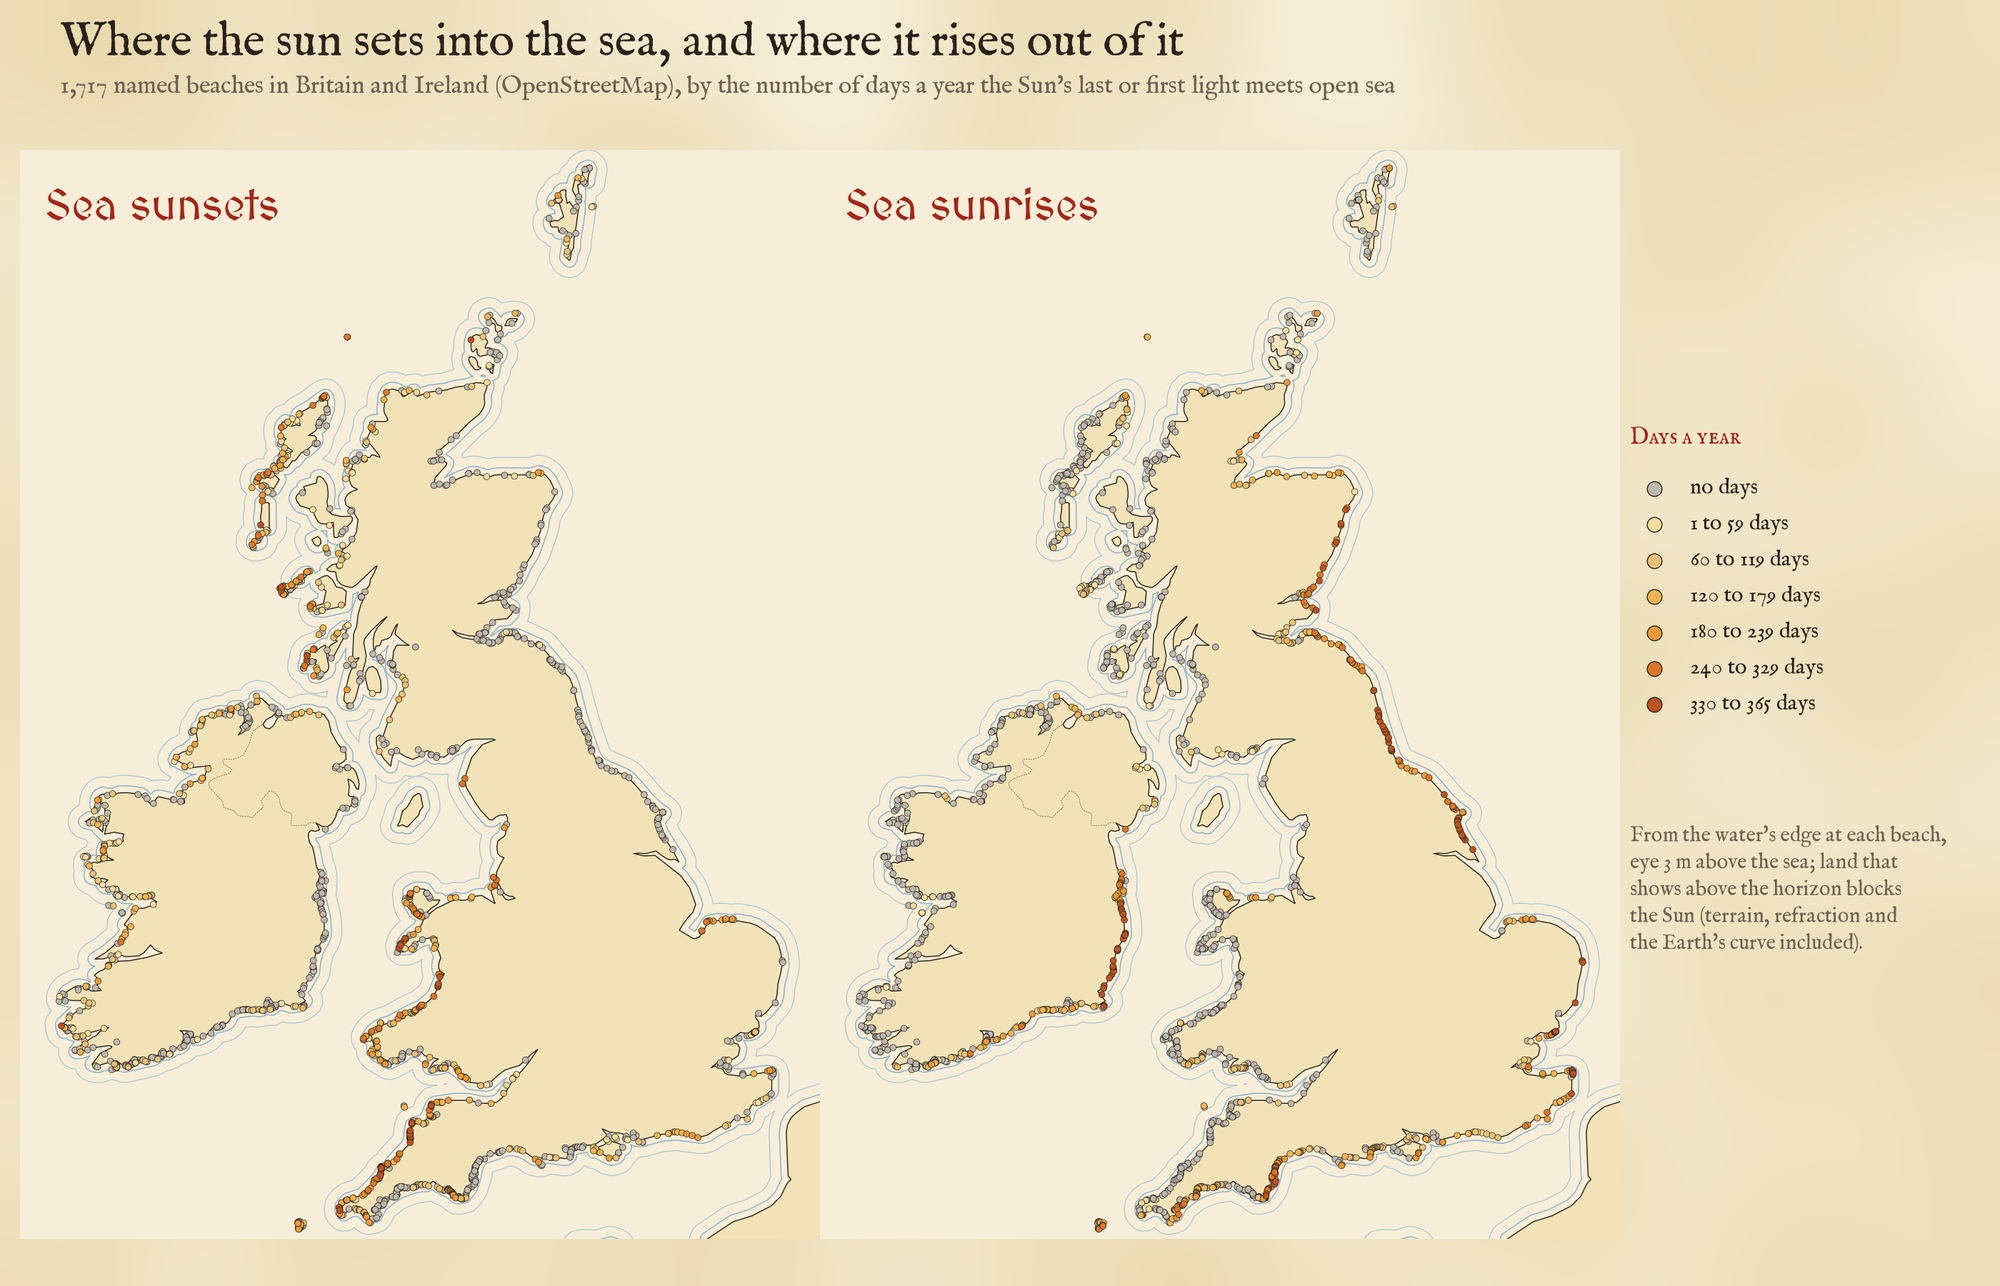
\includegraphics[width=\textwidth]{f_maps.png}
\caption{Days of 2026 with a sunset into, and a sunrise out of, open sea at each beach.}\label{fig:maps}\end{figure}

\subsection{Through the year}
The share of beaches with a sea sunrise varies most through the year, from a winter high to a summer low; the share with a sea sunset is nearly flat (Figure~\ref{fig:calendar}). On 21 December 349 beaches have a sea sunset and 405 a sea sunrise; on 21 June, 303 and 231. 281 beaches have a sea sunset at midwinter but not at midsummer, and 235 the reverse. Figure~\ref{fig:roses} shows four beaches: open Atlantic all year at Sennen Cove, sunrise only at Longsands, Arran in the way at Troon and Lundy at Woolacombe.

\begin{figure}[tbp]\centering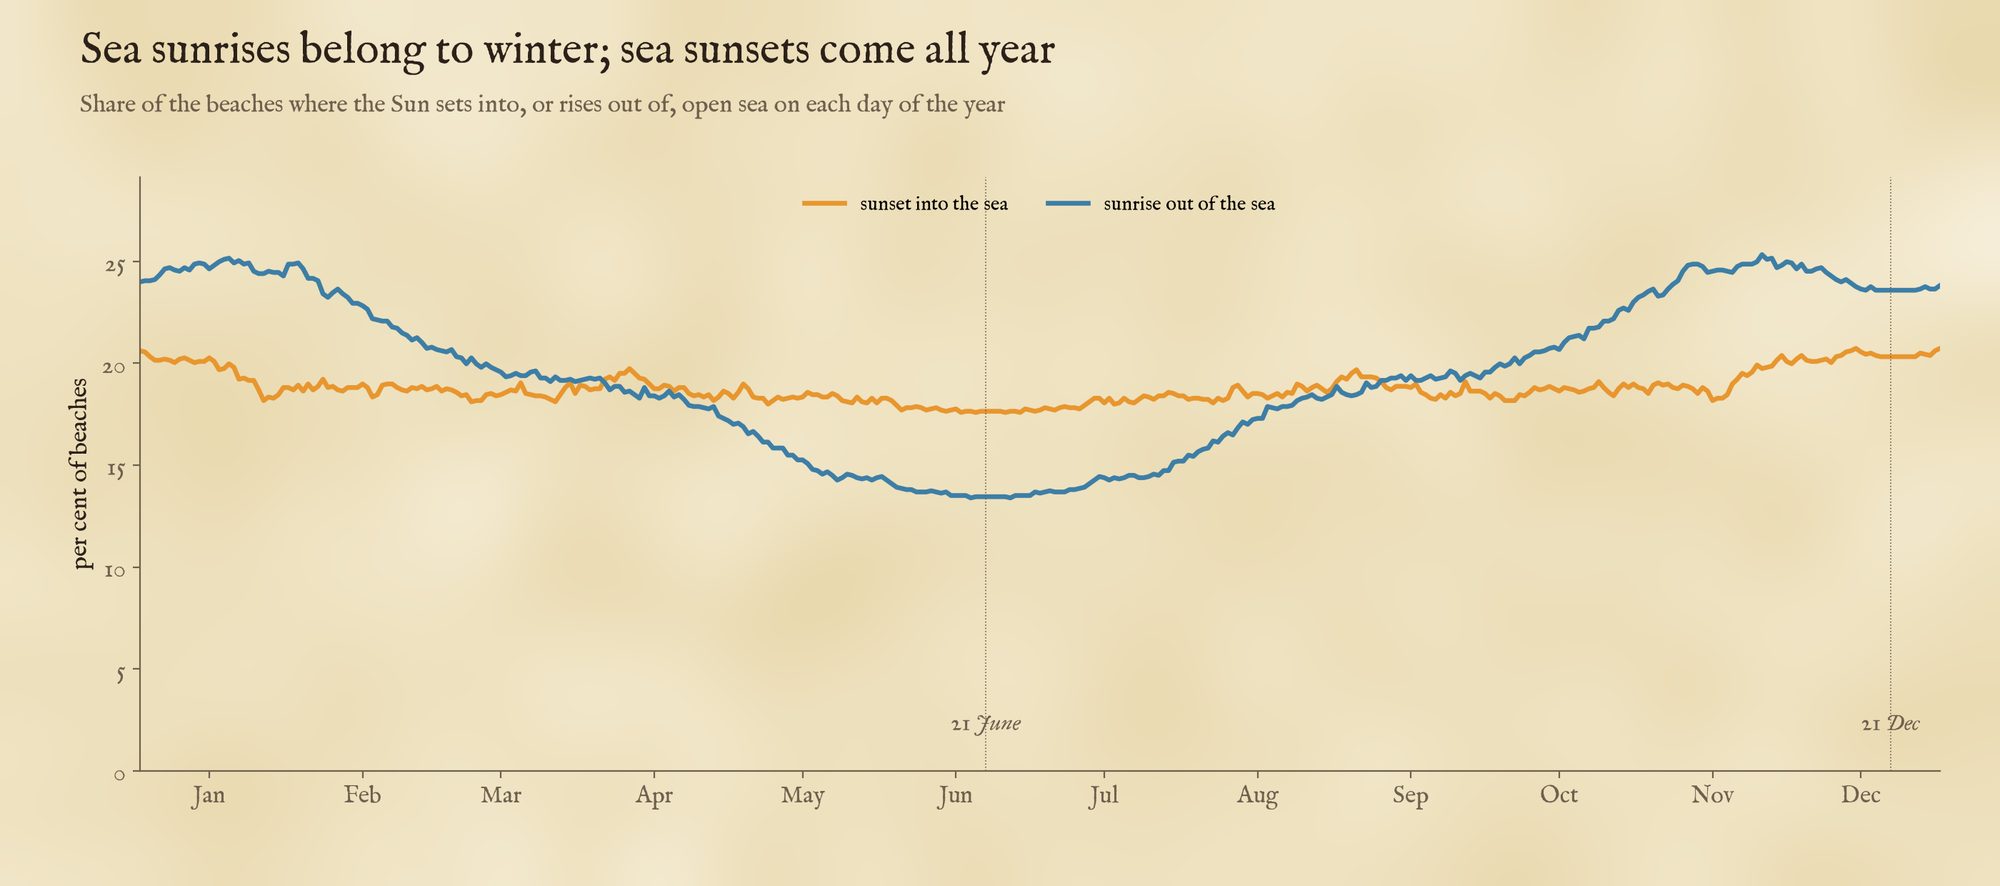
\includegraphics[width=\textwidth]{f_calendar.png}
\caption{Share of beaches with a sea sunset or sunrise on each day of 2026.}\label{fig:calendar}\end{figure}

\begin{figure}[tbp]\centering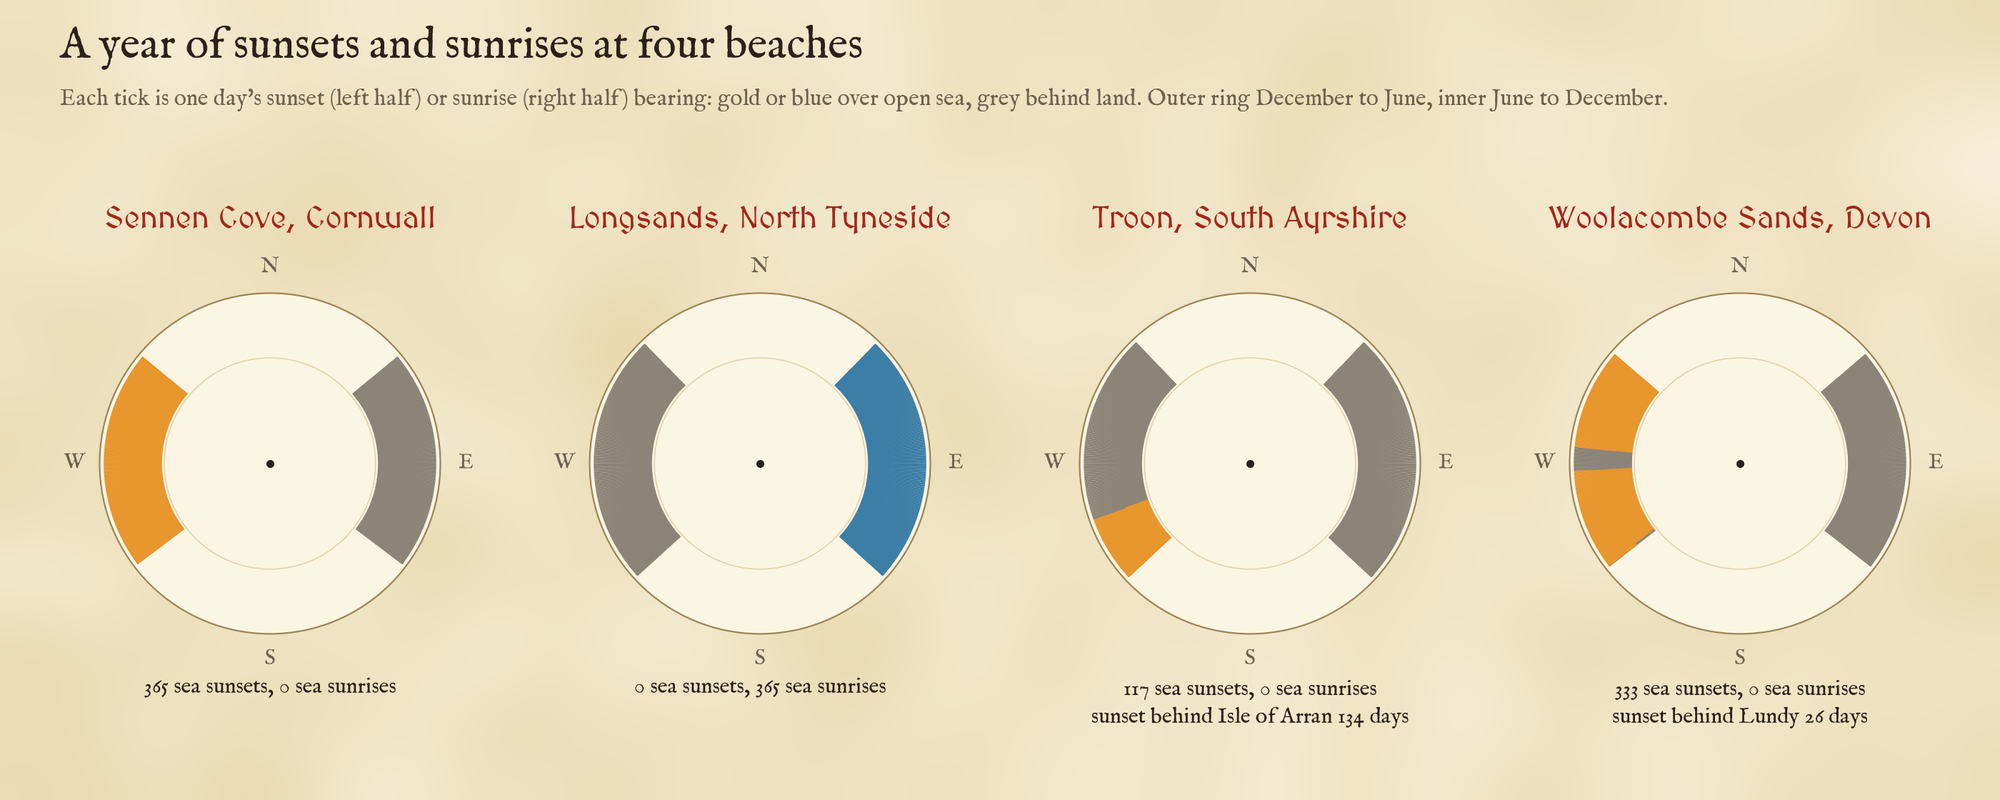
\includegraphics[width=\textwidth]{f_roses.png}
\caption{Sunset and sunrise bearings through the year at four beaches; gold and blue over open sea, grey behind land.}\label{fig:roses}\end{figure}

\subsection{Islands}
Islands hide the Sun on at least one day from 303 beaches at sunset and 179 at sunrise (Table~\ref{tab:islands}, Figure~\ref{fig:islands}). The Isle of Wight and Mull each affect 31 beaches, more than any other island: the Isle of Wight along the Solent and the Sussex coast, Mull from Tiree, Coll and Iona at sunrise and around Oban at sunset. Arran hides the sunset from Troon on 134 days (Figure~\ref{fig:clyde}); Lundy from Woolacombe on 26 days and from Croyde on 28, around the equinoxes; the Isle of Man from Fleswick Bay on 44 days and the sunrise from Gilpin Harbour in County Down on 73. Most blocked days, though, are blocked by the beach's own coast: 90\% of blocked sunsets.

\begin{table}[tbp]\centering\footnotesize\caption{Islands that hide the Sun: beaches and beach-days at sunset and sunrise, and the beach most affected (days).}\label{tab:islands}\begin{tabular}{lrrrrl}\toprule Island & Sunset beaches & Days & Sunrise beaches & Days & Most affected\\\midrule
Isle of Wight & 10 & 1,063 & 21 & 1,362 & East Winner (171)\\
Isle of Mull & 8 & 416 & 23 & 2,089 & Tràigh Mhòr (365)\\
Lewis and Harris & 16 & 699 & 10 & 1,649 & Corran Rà (365)\\
Jura & 5 & 539 & 21 & 764 & Queen's Bay / Loch Staosnaig (234)\\
Lundy & 19 & 513 & 0 & 0 & Peppercombe Beach (58)\\
Skye & 12 & 904 & 6 & 236 & Redpoint Beach (150)\\
Scarba & 0 & 0 & 15 & 116 & Ardalanish Beach (27)\\
Isle of Arran & 10 & 1,359 & 5 & 939 & Grogport Beach (300)\\
Ulva & 1 & 31 & 13 & 244 & Tràigh na Crìche (69)\\
Barra & 14 & 202 & 0 & 0 & Coilleag a' Phrionnsa (90)\\
Iona & 1 & 5 & 12 & 93 & Tràigh Mhòr (20)\\
Eigg & 7 & 299 & 6 & 95 & Port na Murrach/Rhu Beach (76)\\
Islay & 9 & 826 & 4 & 83 & Traigh nam Feannag (347)\\
Mingulay & 12 & 60 & 0 & 0 & Clachan Torra Shoghaigir (9)\\
Lunga & 1 & 27 & 11 & 67 & Black Beach (27)\\
\bottomrule\end{tabular}\end{table}

\begin{figure}[tbp]\centering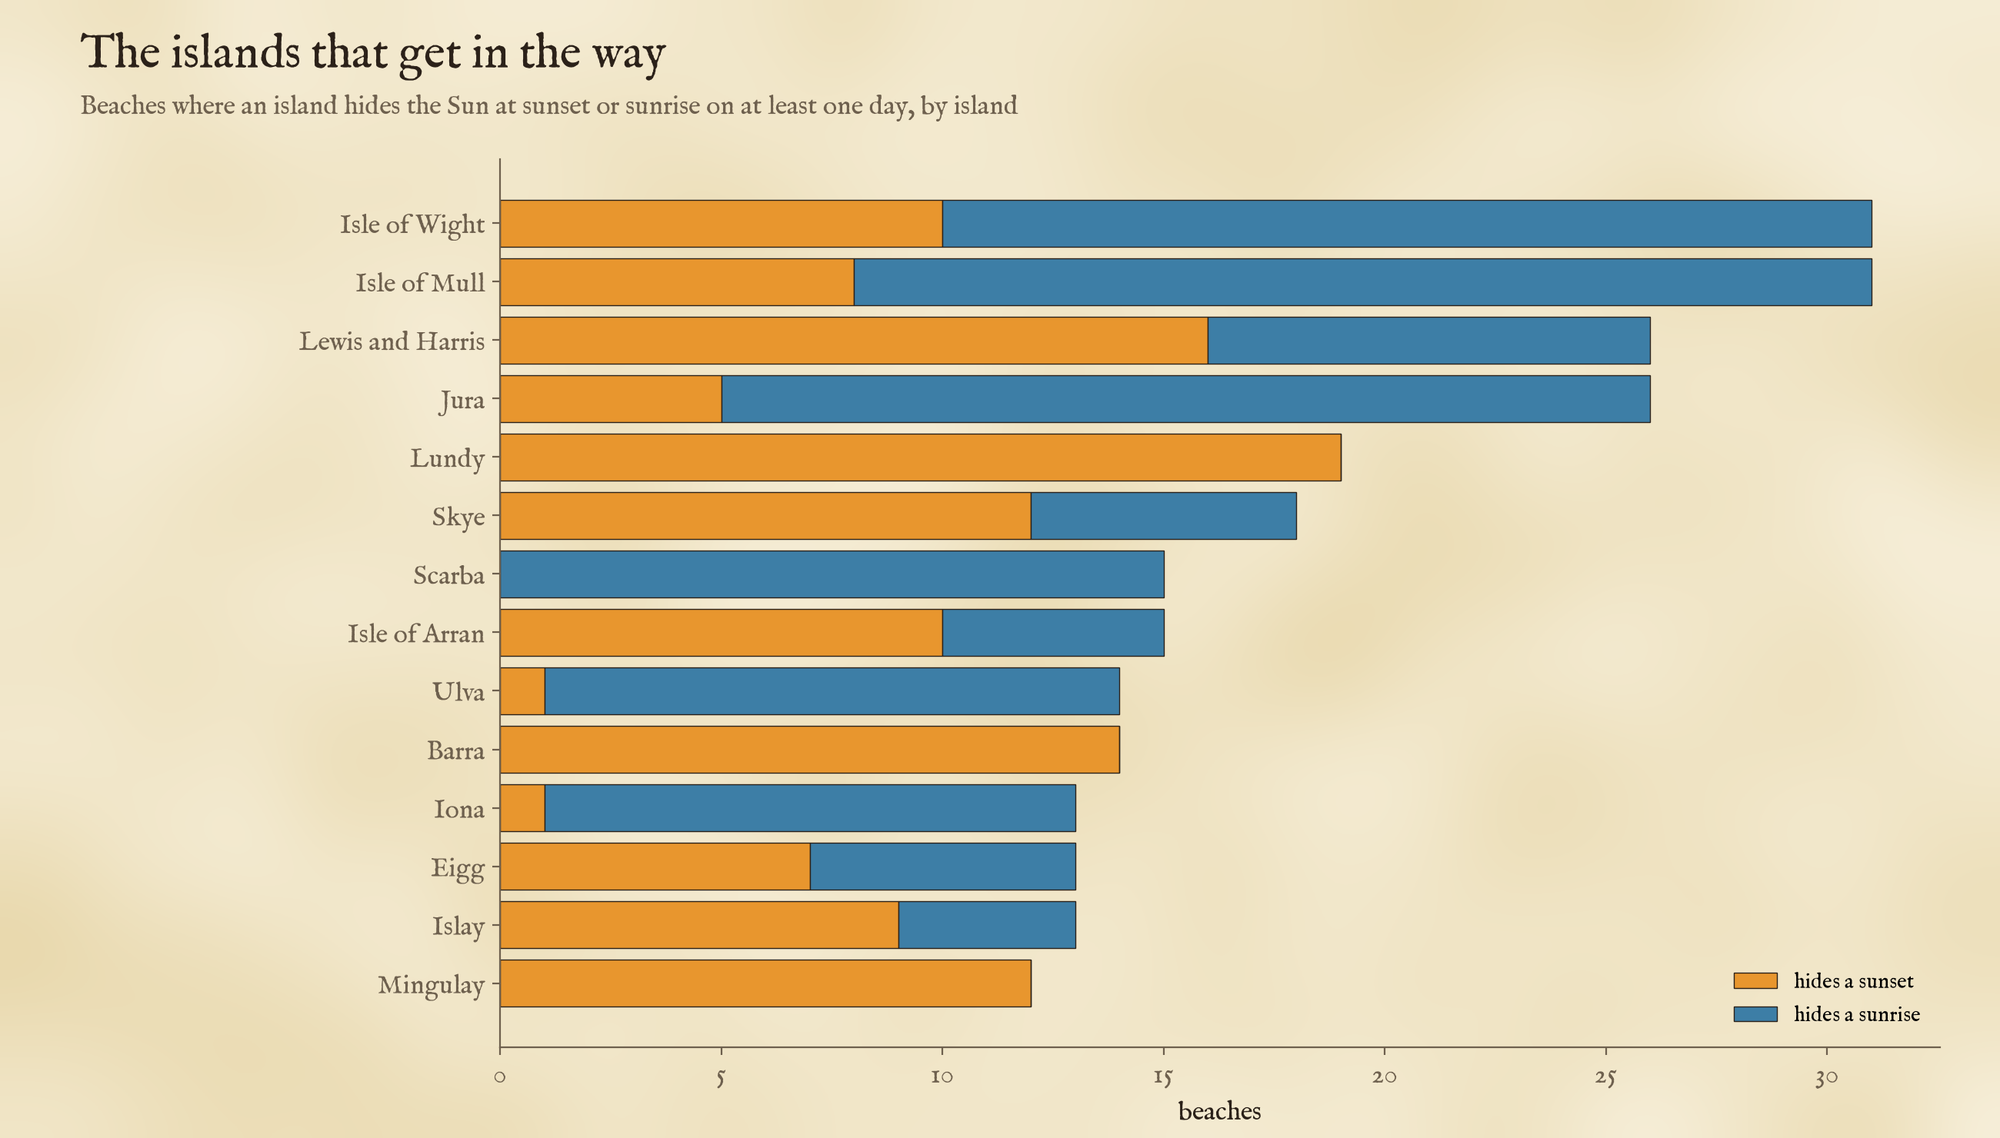
\includegraphics[width=\textwidth]{f_islands.png}
\caption{Islands by the number of beaches from which they hide the sunset or sunrise on at least one day.}\label{fig:islands}\end{figure}

\begin{figure}[tbp]\centering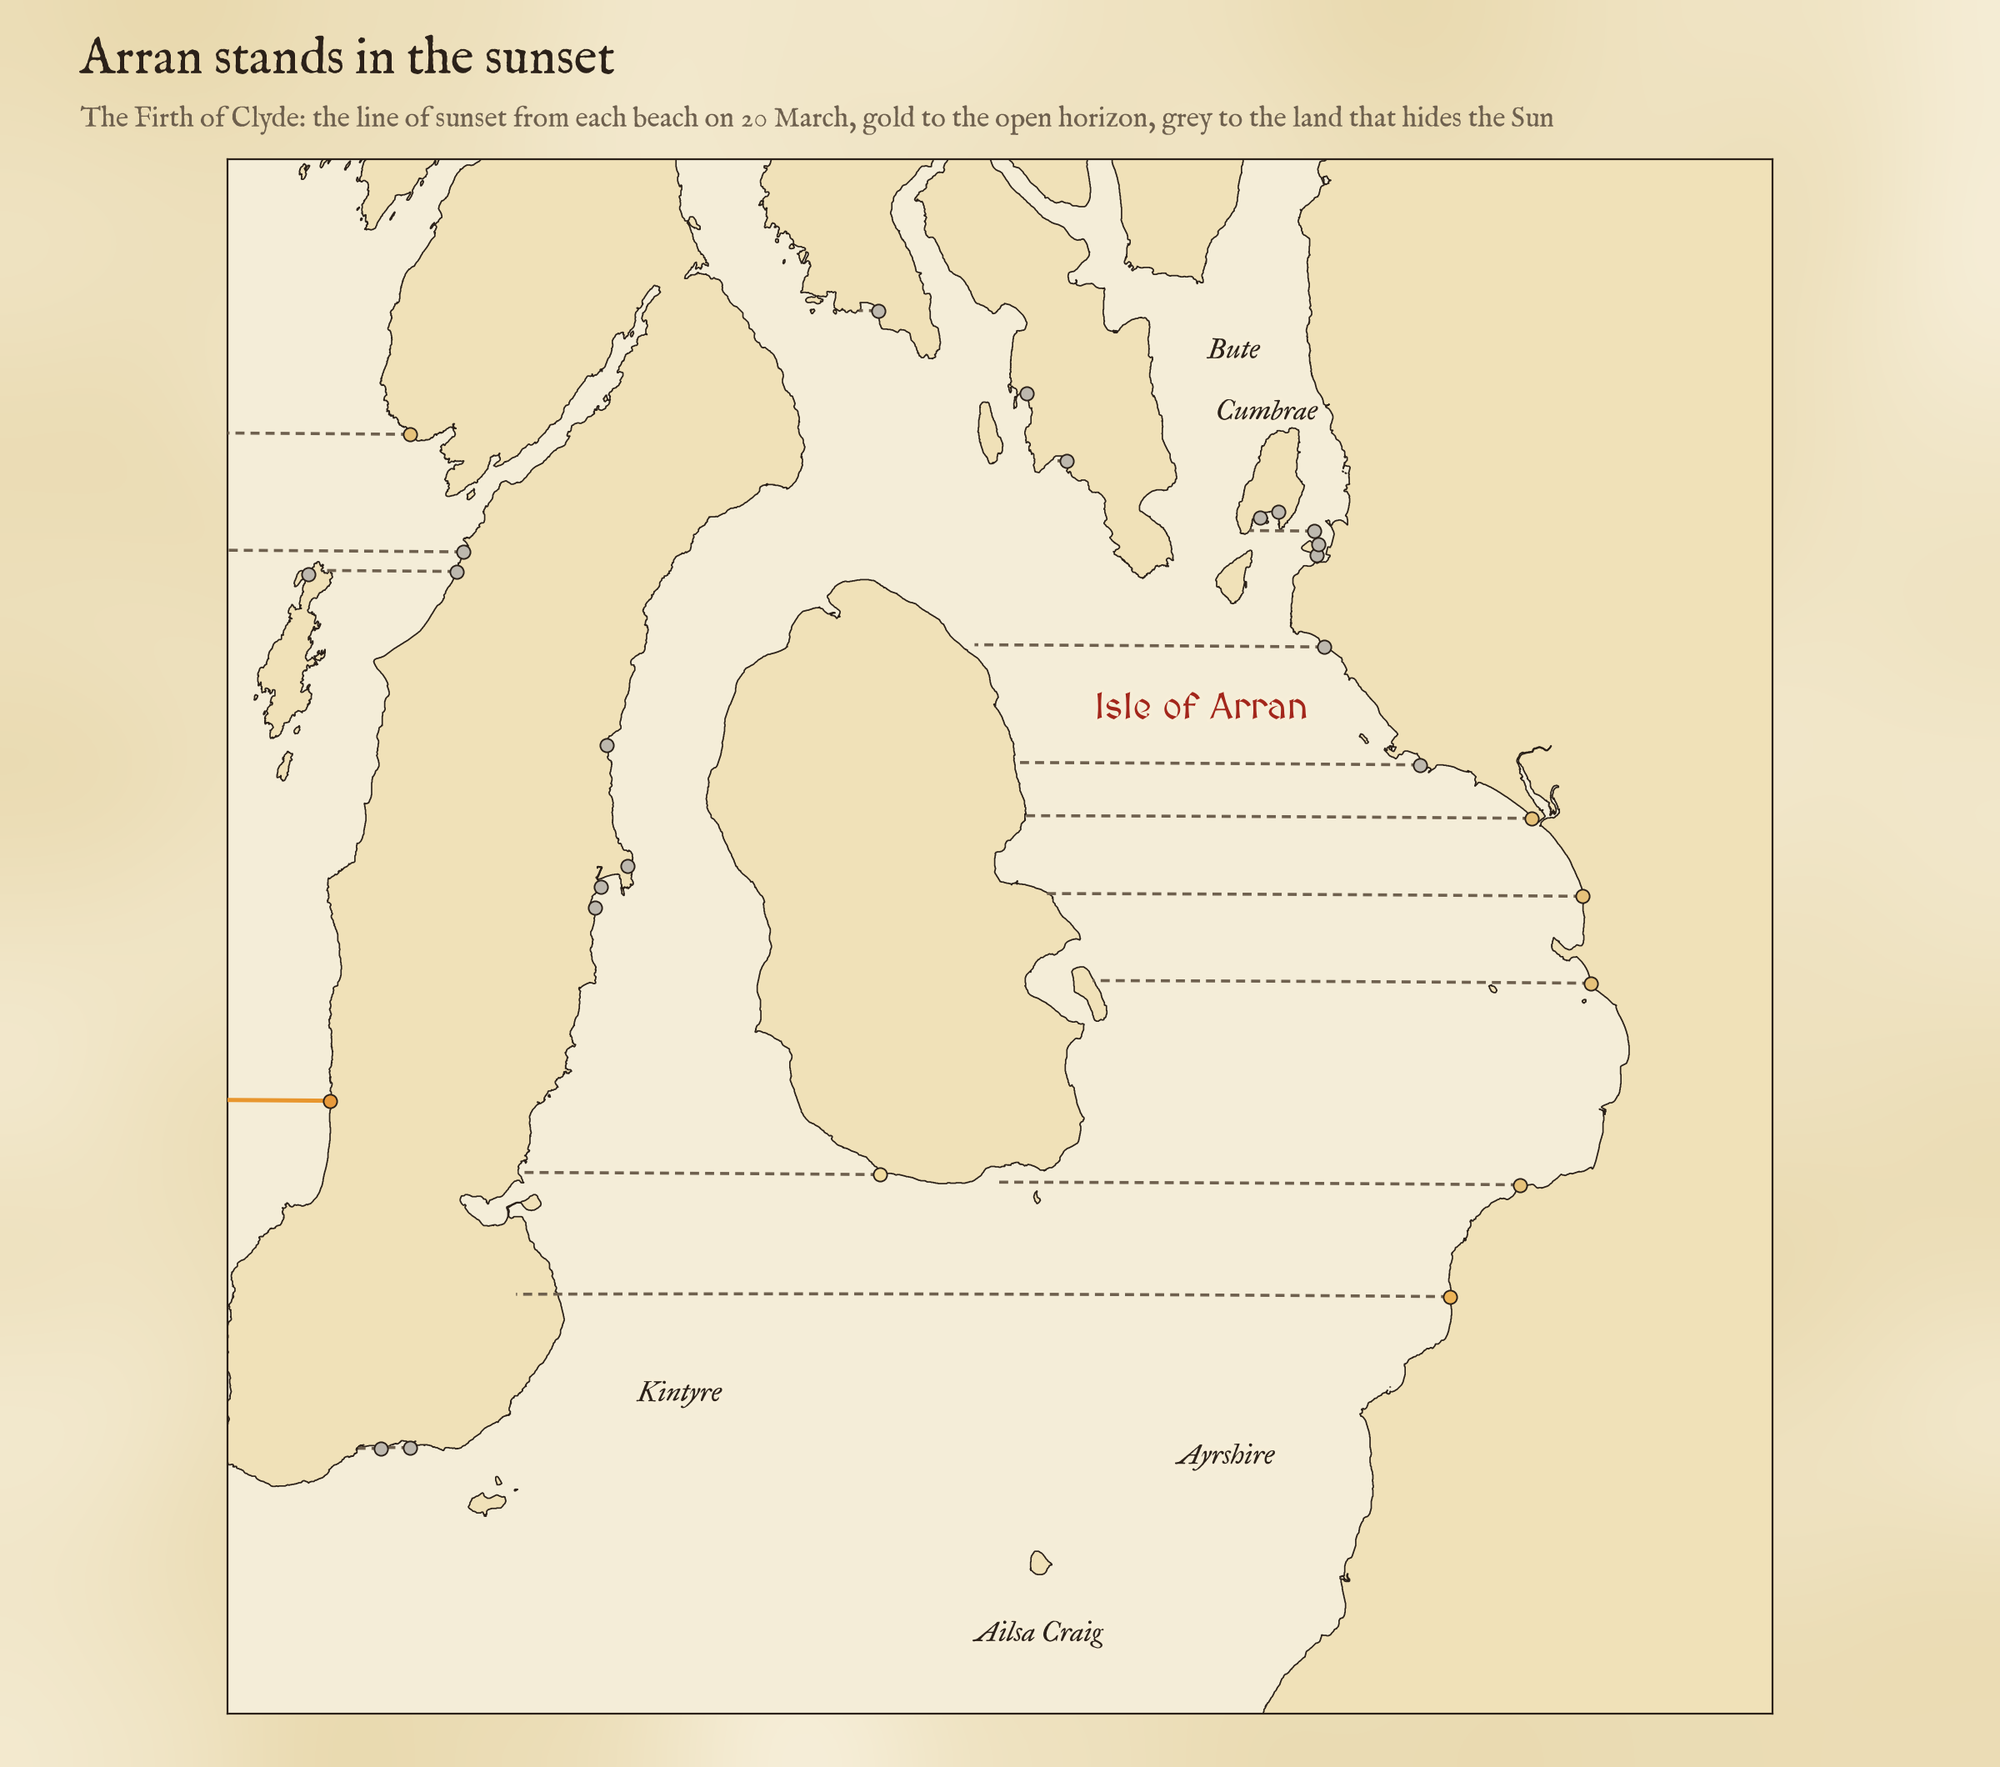
\includegraphics[width=0.95\textwidth]{f_clyde.png}
\caption{The Firth of Clyde: lines of sunset on 20 March from each beach, on the rasterised sea mask.}\label{fig:clyde}\end{figure}

\begin{figure}[tbp]\centering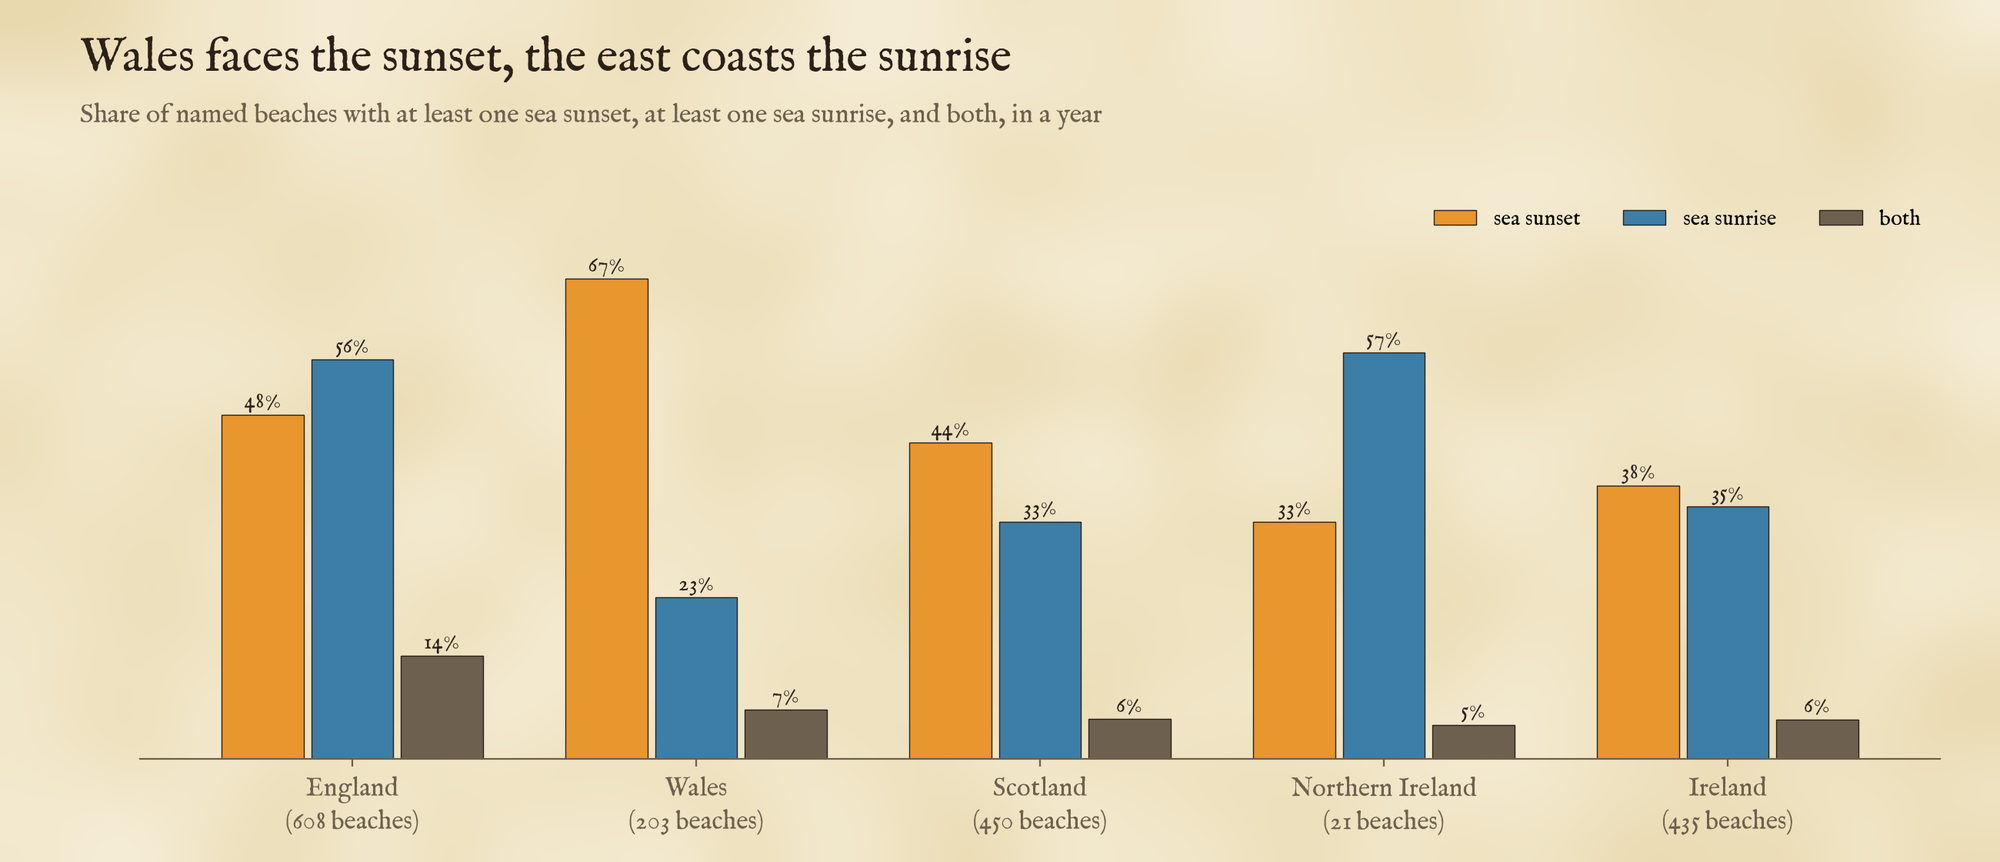
\includegraphics[width=\textwidth]{f_nations.png}
\caption{Share of beaches with a sea sunset, a sea sunrise, or both, by nation.}\label{fig:nations}\end{figure}

\begin{table}[tbp]\centering\scriptsize\caption{Some well-known beaches: days of 2026 with a sea sunset and sunrise, and whether the Sun sets or rises over the sea on the solstices.}\label{tab:cases}\begin{tabular}{llrrcccc}\toprule Beach & County & Sunsets & Sunrises & Set 21 Jun & Set 21 Dec & Rise 21 Jun & Rise 21 Dec\\\midrule
Sennen Cove & Cornwall & 365 & 0 & yes & yes & no & no\\
Fistral Beach & Cornwall & 304 & 0 & yes & no & no & no\\
Porthcurno & Cornwall & 0 & 123 & no & no & no & yes\\
Longsands & North Tyneside & 0 & 365 & no & no & yes & yes\\
Troon & South Ayrshire & 117 & 0 & no & yes & no & no\\
Woolacombe Sands & Devon & 333 & 0 & yes & no & no & no\\
Croyde Beach & Devon & 275 & 0 & yes & no & no & no\\
Fleswick Bay & Cumbria & 280 & 0 & no & yes & no & no\\
Crosby Beach & Sefton & 262 & 0 & yes & no & no & no\\
Half Moon Bay & Lancashire & 215 & 0 & no & yes & no & no\\
Killiney Beach & Dún Laoghaire-Rathdown & 0 & 365 & no & no & yes & yes\\
Dollymount Strand & Dublin & 0 & 183 & no & no & no & yes\\
Inch Beach & Kerry & 94 & 0 & no & no & no & no\\
Keem Beach & Mayo & 0 & 0 & no & no & no & no\\
Lahinch Beach & Clare & 175 & 0 & no & yes & no & no\\
Gilpin Harbour & Down & 0 & 111 & no & no & no & yes\\
Brighton Beach & Brighton and Hove & 147 & 109 & no & yes & no & yes\\
Rhossili Bay Beach & Swansea & 202 & 0 & no & yes & no & no\\
Whitesands Beach & Pembrokeshire & 234 & 0 & yes & no & no & no\\
Botany Bay & Kent & 196 & 341 & yes & no & yes & no\\
Saltburn Sands & Redcar and Cleveland & 0 & 187 & no & no & yes & no\\
Durdle Door & Dorset & 9 & 117 & no & no & no & yes\\
\bottomrule\end{tabular}\end{table}


\subsection{Checks by eye}
I checked a handful of well-known beaches against the map and the expected geometry before reading any totals. Sennen Cove, facing the open Atlantic west of Land's End, has a sea sunset on all 365 days. Fistral at Newquay faces north-west and gets 304 sea sunsets, but not at midwinter, when the sunset bearing of about 230\textdegree{} crosses its own headland. Longsands at Tynemouth and Killiney in County Dublin face east and get a sea sunrise on every day and no sea sunset, as expected; Dollymount Strand, inside Dublin Bay, loses half its sunrises to Howth (183 days). Keem Bay on Achill opens to the south-east under high cliffs and gets neither, which matches its setting. Inch in Kerry looks across Dingle Bay to the Iveragh peninsula and gets sea sunsets only around the equinoxes (94 days). Troon and Woolacombe show Arran and Lundy in the expected directions (Figure~\ref{fig:clyde}). For each of these I also drew the rays over the rasterised sea mask to confirm the observer point and the blocking land.

\section{Discussion}
Three things decide whether a beach has a sea sunset: which way it faces, how far the sunset bearing swings across its view in a year, and what stands at the ends of that view. Only a beach facing between about west-south-west and west-north-west on an open coast, like the Atlantic coasts of Cornwall, gets one every day; most west-facing beaches lose part of the year to their own headlands or to the far side of a bay, and the result is often a season of sea sunsets rather than a year of them. The curvature of the Earth matters as much as the coastline: a low island 40 or 50 km away is below the sea horizon and does not hide the Sun, while the mountains of Arran or the Isle of Man do. Winter favours sea views because the Sun then rises and sets further south, across the open water that many south-facing beaches look onto, while at midsummer it sets far to the north-west, along the coast.

\section{Limitations}
The coastline is OpenStreetMap's mean high water line, so at low tide on wide sands the foreground is beach, not sea. Rasterising at zoom 10 smooths features below about 50 m, so very small rocks and stacks are missed, while terrain at 90 m can smear land a little out to sea in the far field. Refraction near the horizon varies with the weather by up to about half a degree, which can change the result on marginal days, and the clear line of sight says nothing about cloud. The best point along each beach is used; from other points the view may be narrower. Only named beaches in OpenStreetMap are included, so coverage follows the mappers (Blackpool's main beach, for example, has no name in the data). Beyond the terrain tiles (south of about 49.6\textdegree N and east of 2.1\textdegree E) far land is not modelled, which matters little because it lies more than 150 km from most beaches.

\section{Data availability}
The interactive map is at \url{https://maps.tristanhotham.com/sea-sunsets/}; data and code at \url{https://github.com/Tristan-Hotham/sea-sunsets}. \texttt{beaches.csv} gives every beach with its observer point, counts and day-by-day strings; \texttt{results.json} every number in this paper. Data derived from OpenStreetMap are under the Open Database Licence; text and figures CC BY 4.0; code MIT.

\section*{AI assistance}
I wrote the text, with drafting and editing assistance from Claude (Anthropic), which also helped prepare the analysis code. I reviewed and checked all text and results.

\begin{thebibliography}{9}
\bibitem[Bast and Buchhold(2017)]{qlever} Bast, H. and Buchhold, B. (2017) QLever: a query engine for efficient SPARQL+Text search. \textit{Proceedings of the 2017 ACM Conference on Information and Knowledge Management (CIKM)}, 647-656.
\bibitem[OpenFreeMap(2026)]{openfreemap} OpenFreeMap (2026) Vector tiles of OpenStreetMap in the OpenMapTiles schema. \url{https://openfreemap.org/}
\bibitem[OpenStreetMap(2026)]{osm} OpenStreetMap contributors (2026) OpenStreetMap. Open Database Licence. \url{https://www.openstreetmap.org/}
\bibitem[Spencer(1971)]{spencer1971} Spencer, J. W. (1971) Fourier series representation of the position of the sun. \textit{Search} 2(5), 172.
\end{thebibliography}
\end{document}
